A neural network is a machine learning model and can be seen as a universal function approximator. A function approximator approximates a function. This function maps an input $X$ to an output $Y$.\autocites{Hornik.1989}{Ertel.2016}
In consequence, a neural network itself can be seen as a function. 
A neural network is structured in layers. \autocite{Ertel.2016}  A layer receives an input and returns an output. The first layer is called input layer, the last layer is called output layer, and the remaining layers are called hidden layers. \autocite{LeCun.2015b} A hidden layer is a layer which receives the output of its previous layer or previous layers as input. The input layer is the layer receiving the input of the neural network. The output layer is the layer returning the output of the neural network. This is illustrated in Figure~\ref{img:neuralnetwork}.
This way, layers themselves can be seen as functions. Hence, a neural network can be described as a chain of layer functions. Given the layer~$F_l$ at position~$l$, the input~$X$, and the output~$Y$ of the neural network~$F$, then $Y$ is computed as defined by Equation~\eqref{eq:neuralnetwork}.
\begin{equation}
	\label{eq:neuralnetwork}
	Y = F(X) = F_l(F_{l-1}\dots(F_1(X)\dots)) 
\end{equation}
\begin{figure}[H]
	\centering
	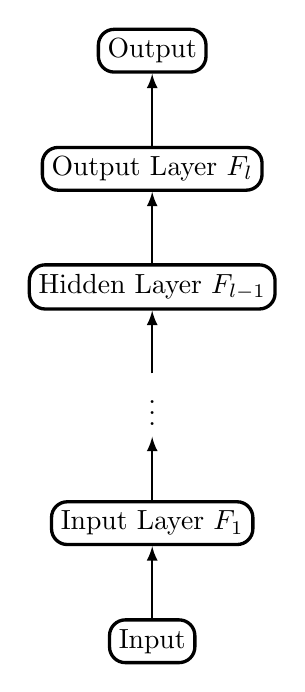
\begin{tikzpicture}[
	cell/.style={
		rectangle, 
		rounded corners=2mm, 
		draw,
		very thick,
		align=center,
	},
	ArrowC1/.style={% Arrows with rounded corners
		rounded corners=.25cm,
		thick,
	},
]
	\node [cell] (out) at (0,7.5) {Output};
	\node [cell] (fl) at (0,6) {Output Layer $F_l$};
	\node [cell] (fl1) at (0,4.5) {Hidden Layer $F_{l-1}$};
	\node [very thick, align = center](dots) at (0,3) {\vdots};
	\node [cell] (f1) at (0,1.5) {Input Layer $F_1$};
	\node [cell] (in) at (0,0) {Input};
	
	\draw [-latex,ArrowC1] (fl) -- (out);
	\draw [-latex,ArrowC1] (fl1) -- (fl);
	\draw [-latex,ArrowC1] (dots) -- (fl1);
	\draw [-latex,ArrowC1] (f1) -- (dots);
	\draw [-latex,ArrowC1] (in) -- (f1);
\end{tikzpicture}
	\caption{Neural Network (own figure)} \label{img:neuralnetwork}
\end{figure}
A layer consists of neurons. Neurons are the basic processing units of neural networks. A neuron consists of $n$ weighted connections $w_i, i \in [1;n]$, a sum function $\sum$, and an activation function $\varphi$, see Figure \ref{img:neuron}. Each connection is connected to an input of the neuron. The sum function sums the weighted inputs. The activation function transforms the sum. The result of the activation function is the output $y$ of the neuron. \autocite{Ertel.2016} Given an input $x$, $y$ is computed as defined by Equation \eqref{eq:neurn}.
\begin{equation}
	\label{eq:neurn}
	y = \varphi(\sum x \cdot w)
\end{equation}
\begin{figure}[H]
	\centering
	\begin{tikzpicture}[
cell/.style={
	rectangle, 
	rounded corners=2mm, 
	draw,
	very thick,
	align=center,
},
ArrowC1/.style={% Arrows with rounded corners
	rounded corners=.25cm,
	thick,
},
]
	\node (x0) at (0,3) {$x_0$};
	\node (x1) at (0,2) {$x_1$};
	\node (..) at (0,1) {$\vdots$};
	\node (xn) at (0,0) {$x_n$};
	\node[draw, circle, minimum size=1cm] (sum) at (2,1.5) {$\sum$};
	\node[draw, circle, minimum size=1cm] (phi) at (4,1.5) {$\varphi$};
	\node (y) at (6,1.5) {$y$};
	\draw[-latex,ArrowC1] (x0) -- (sum) node[sloped,pos=.3,above] {$w_0$};
	\draw[-latex,ArrowC1] (x1) -- (sum) node[sloped,pos=.3,above] {$w_1$};
	\draw[-latex,ArrowC1] (xn) -- (sum) node[sloped,pos=.3,above] {$w_n$};
	\draw[-latex,ArrowC1] (sum) -- (phi);
	\draw[-latex,ArrowC1] (phi) -- (y);
	\node[draw,	ellipse, minimum height=2cm,minimum width=3cm, label=Neuron] (neuron) at (3,1.5) {};
	\end{tikzpicture}
	\caption{Neuron (own figure)} \label{img:neuron}
\end{figure}
